\documentclass[12pt]{report}

%\usepackage[french]{babel}
\usepackage[utf8]{inputenc}%pour le é 
\usepackage[T1]{fontenc}
\usepackage{fancyhdr}%pour l'en-tete 
\usepackage{graphicx}%pour les images
\usepackage[margin=1in]{geometry}
\usepackage{cite}%pour bibliographie 
\usepackage{wrapfig} %pour figure a coté du texte
%\frenchbsetup{StandardLists=true} % à inclure si on utilise \usepackage[french]{babel}
\usepackage{enumitem}
\usepackage{amssymb}
\usepackage[section]{placeins}
\usepackage{glossaries}


\usepackage{subcaption}
%		Header		%		
\usepackage{fancyhdr}
\pagestyle{fancy}
\rhead{\thepage}
\lhead{\leftmark}

\usepackage{makeidx}
\makeindex

\makeglossaries
 
\newglossaryentry{MSA}
{
    name=MSA,
    description={Modern Standard Arabic. }
}

\newglossaryentry{CA}
{
    name=CA,
    description={Classical Arabic. }
}

\newglossaryentry{DA}
{
    name=DA,
    description={Dialectal Arabic. }
}

\input{Parts/commands.tex}



\begin{document}
\input{Parts/remerciements.tex}
\input{Parts/resume.tex}
\listoffigures  % table des figures



\tableofcontents
\newpage
\chapter{Introductions génerale}
\chapter{Les robots mobiles autonomes}
\section{Description d'un robot mobile autonome}
AGV, AMR, Cobots, robots mobiles, exosquelettes, robots collaboratifs … la robotique industrielle est devenue un vaste domaine dans lequel il n’est pas évident de se repérer. Cet article traite de la notion de Robot Mobile Autonome, dit AMR.

\begin{figure}[h]
    \centering
    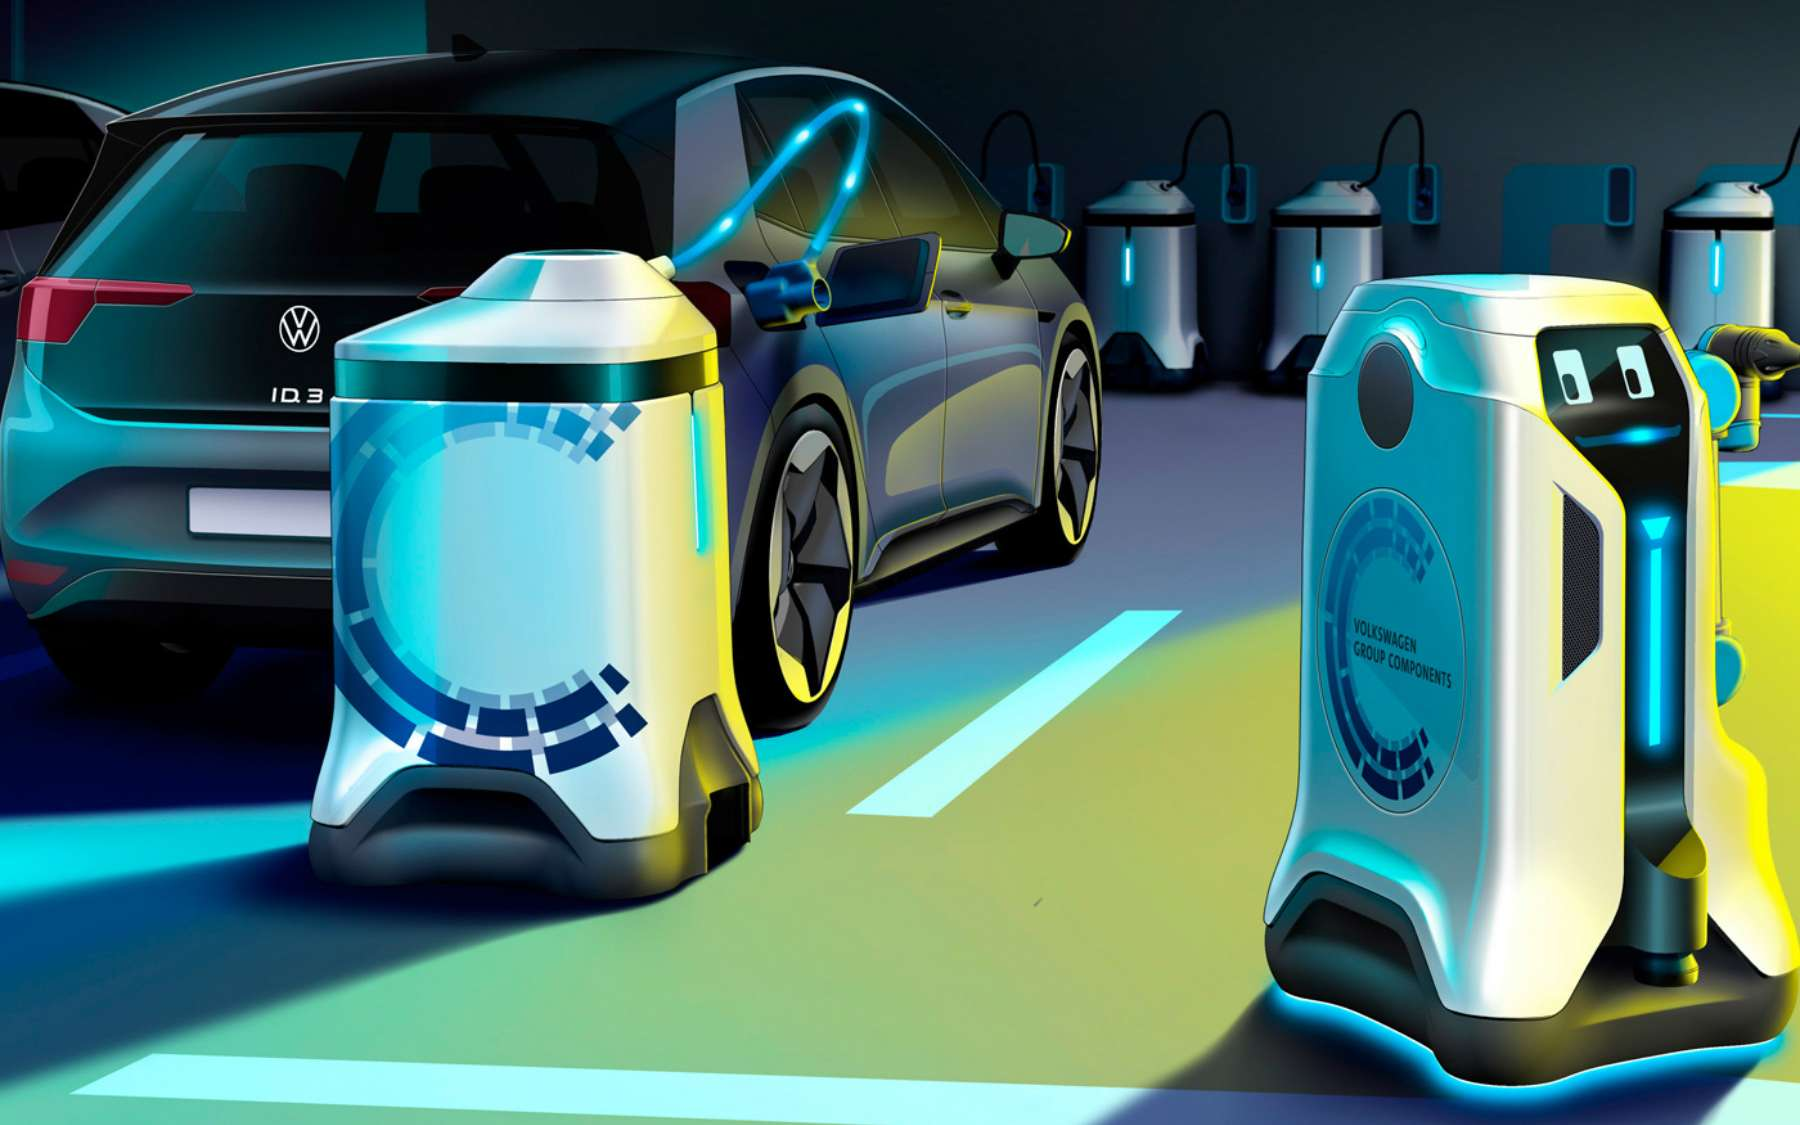
\includegraphics[width=14cm]{assets/robot_autonome.jpg}
    \caption{Robot mobile pour recharger les vehicules electriques \cite{DescriptionRobotMobile}}
    \label{Tux}
    \end{figure}

L’AMR est un robot collaboratif dans le sens où il fonctionne au plus proche des opérateurs. Ils opèrent au milieu des Hommes et des Machines, au coeur des zones de travail et dans les univers encombrés.

L’AMR est doté d’un haut degré d’autonomie, il peut se déplacer dans un environnement plus ou moins vaste sans l’intervention humaine. Il se déploie facilement et s’adapte à la configuration d’un site, ne nécessitant pas de modification coûteuse d’infrastructure. De même, si l’infrastructure et le besoin viennent à évoluer, les robots peuvent être reprogrammés facilement. Enfin, ce type de robots permet d’automatiser les tâches de transport et le déplacement de marchandises à l’intérieur d’un bâtiment, et constitue une solution agile pour la transformation vers l’Usine 4.0 et la supply chain digitalisée. Le robot mobile autonome est donc le symbole d’une mobilité industrielle nouvelle génération.
\begin{figure}[h]
    \centering
    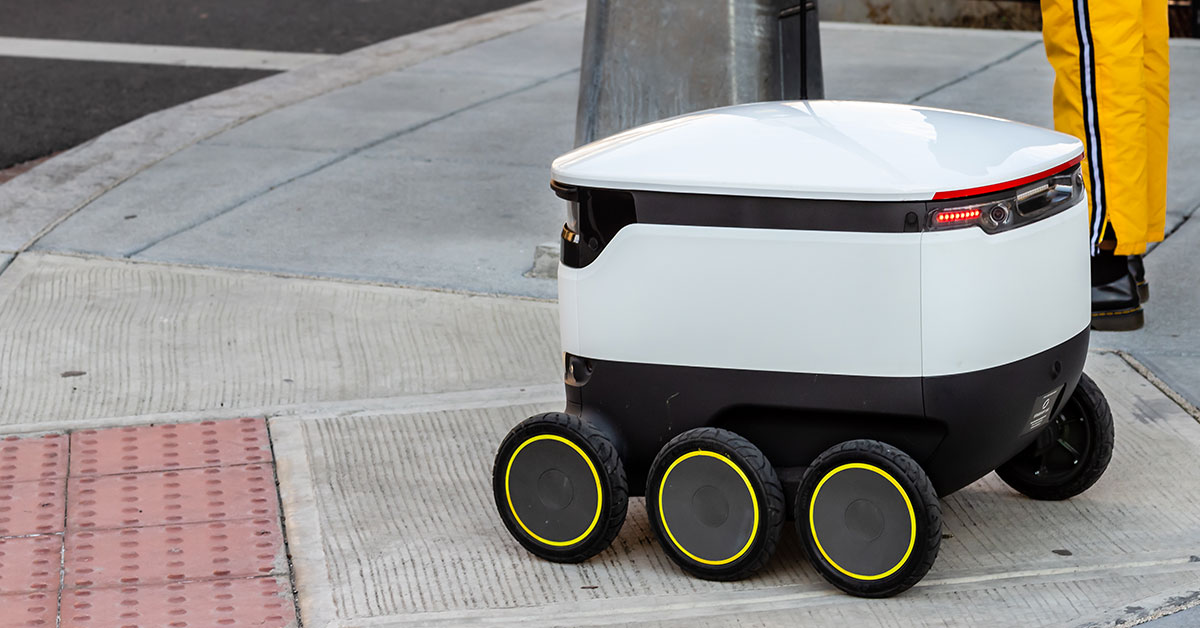
\includegraphics[width=14cm]{assets/Robot_AMR.jpg}
    \caption{Exemple d'un robot autonome pour la livraison \cite{italianingenioMobiliteIndustrieRobots2021}}
    \label{amr}
    \end{figure}
\subsection{Quelles différences entre un AMR et un AGV ?
}
Contrairement aux AGV (Automated Guided Vehicle) qui ont des trajectoires dédiées, les AMR sont totalement libres et s’adaptent aux environnements dynamiques. L’AGV est guidé par des rails ou repères au sol, tandis que l’AMR navigue en total autonomie dans un environnement cartographié au préalable. Les robots mobiles autonomes sont dotés de technologies de pointe leur permettant de naviguer avec précision dans un périmètre donnée, d’éviter les obstacles et d’évoluer sans risque de collision. La notion de sécurité est un sujet auquel les constructeurs sont particulièrement vigilants, de part les nombreuses interactions entre l’homme et la machine.
\section{Classification des robots mobiles}
La classification des robots se fait selon plusieurs critères.
 \begin{itemize}    
     \item Le degré d’autonomie.     
     \item Le domaine d’application.    
      \item  Le système de locomotion. 
\end{itemize}
\newpage
Il est important de noter que l’expression « robots mobiles » bien que désignant l’ensemble des robots à base mobile (par opposition aux robots manipulateurs), est généralement employé afin de désigner les robots mobiles terrestres.
%https://www.ummto.dz/dspace/bitstream/handle/ummto/7333/HamoudiAhcene.pdf
\subsection{Classification selon le degré d'autonomie}
Un robot autonome  doté de capacités décisionnelles et de moyens d’acquisition et de traitements de données lui permettant d’accomplir sous contrôle humain réduit voire même absent un certain nombre de tâches, dans un environnement connu ou non, donc on peut classer les robots mobiles de la manière suivante :

\subsubsection{Robot télécommandé}
Ce sont des robots commandé par un opérateur (machines ou être humain), qui leurs dicte chaque tâche élémentaire à accomplir (avancer, reculer, tourner, etc.).
\subsubsection{Robot semi-autonome}
Ces types de robots effectuent un certain nombre d’opérations par eux même d’une façon complètement autonome mais il peut être interrompu dans n'importe quel momment pour recevoir de nouvelles commandes dictées par l'opérateur .

\subsubsection{Robot autonome}
On dit qu'un  robot est complètement autonome s’il est capable d’adapter son comportement à l’environnement dans lequel il évolue.
L’autonomie est la capacité propre d’un système sans équipage, à capter, percevoir, analyser, communiquer, planifier, et prendre des décisions et agir  les objectifs qupour atteindre lui ont été assignés.

\subsection{Classification selon le domaine d'application}
L’un des plus grands avantages des robots mobiles est le fait que leur domaine d’application est illimité, nous présentons ici quelques domaines d’application :

\subsubsection{Les robots industriels et de service}
La robotique industrielle est  définie par l'ISO comme un contrôle automatique, polyvalent manipulateur programmable dans trois ou plusieurs axes.
Les applications typiques incluent des robots de soudage, de peinture et d'assemblage. La robotique industrielle inspecte les produits, rapidement et précisément.
Les robots industriels sont très utilisés en automobile, leur conception nécessite  un très haut niveau dans le domaine de l'ingénierie.
Quant aux robots de service, ils sont destinés à aider des handicapés, à guider les aveugles ainsi qu’à piloter des voitures automatiques.
\subsubsection{Les robots militaires}
Appelé arme autonome, est un robot autonome contrôlé à distance, conçu pour des applications militaires. Les drones sont une sous-classe des robots militaires.
Ce champ d’application présente l’intérêt de fournir des spécificatins accrues telles la vitesse des véhicules, leurs capacités de franchissement d’obstacles, ainsi que leur rapidité de réaction en font des robots de très hautes performances.
\subsubsection{les robots de laboratoire}
Larobotique de laboratoireest l'utilisation derobotsdans les laboratoires debiologieou de chimie,pour ce la les sociétés pharmaceutiques utilisent des robots pour la synthèse de nouvelles entités chimiques ou pharmaceutiques afin de tester la valeur des matières chimiques.


\subsection{Classification selon le type de locomotion}
\subsubsection{Les robots mobiles à roues}
La mobilité par roues est la structure mécanique la plus utilisée en robotique mobile,Il assure un déplacement aisé, mais nécessite un sol relativement plat. On distingue plusieurs classes de robots à roues, déterminées principalement par la position et le nombre de roues utilisées. Nous citerons ici les classes principales de robots à roues.
\subsubsection{Robots unicycle}
Un robot de type unicycle est actionné soit par une seule roue ou par deux roues indépendantes, on utilise (gyroscope) et  (accéléromètre) pour assurer sa stabilité. Son centre de rotation est situé sur l’axe reliant les deux roues motrices. 
Un robot unicycle celui qui bouge dans un plan 2D ayant une certaine vitesse de déplacement vers l’avant, mais aucun mouvement latéral instantané, car ce type de robots sont un système non-holonome. Ils sont donc incapables d’avoir un déplacement dans une direction perpendiculaire aux roues de locomotion.
\subsubsection{Robots tricycle}
Un robot de type tricycle est constitué de deux roues fixes placées sur un même axe et d’une roue libre  centrée. Le mouvement du robot est alors donné par la vitesse des roues fixes et son orientation est assurée par la roue libre. 
C’est là aussi un robot non-holonome. En effet, il lui est impossible de ce déplacé dans une direction perpendiculaire aux roues fixes.
\subsubsection{robots voiture}
Un robot de type voiture est semblable au robot tricycle, sauf qu’il est constitué de deux roues fixes placées sur un même axe et de deux roues centrées orientables.    Le robot de type voiture est cependant plus stable . Toutes les autres propriétés du robot voiture sont identiques au robot tricycle.L’un des plus grands projets dans ce domaine est le projet développé par « Google » le « Google Self-Driving Car Project ».

image 
\subsubsection{Robots mobiles omnidirectionnels}
Un robot mobile est  omnidirectionnel si l’on peut agir indépendamment sur la vitesse de translation selon les axes x et y et la vitesse de rotation autour de z. En général constitué de trois roues décentrées orientables qui sont placées de manière à former un triangle équilatéral.
L’énorme avantage de ce robot  est qu’il est holonome,Mais ceci ne se fait qu’au dépend d’une complexité mécanique bien plus importante par rapport aux autres types de robots mobiles .
\subsection{Les avantages des différents types de robots }
\subsubsection{Uicycle}
* Stable.
* Rotation sur soi-meme.
* Complexité faible.
\subsubsection*{Tricycle}
* Complexité mécanique modérée.
\subsubsection{Voiture}
* Stable.
* Complexité mécanique modérée.
\subsubsection{Omnidirectionnel}
* Holonome.
* Stable.
* Rotation sur soi-meme.
\subsection{Les inconvénients des différents types de robots}
\subsubsection{Unicycle}
* Non-holonome.
\subsubsection{Tricycle}
* Non-holonome.
* Peu stable.
* Pas de Rotation sur soi-meme.
\subsubsection{Voiture}
* Non-holonome.
* Pas de Rotation sur soi-meme.
\subsubsection{Omnidirectionnel}
* Complexité mécanique importante.
\subsection{Les robots mobiles a chenilles}
Les robots mobiles à chenilles présentent l’avantage d’une bonne adhérence au sol et d’une faculté de franchissement d’obstacles.L’utilisation est orientée vers l’emploi sur sol accidenté ou de mauvaise qualité au niveau de l’adhérence. Généralement ils sont utilisés  principalement pour la surveillance ou de déminage.
image 
\subsection{Les robots humanoïdes}
Les robots marcheurs sont destinés à réaliser des tâches dont l’accès au site est  dangereux ou impossible à un humain. Leur anatomie a de nombreux degrés de liberté, ce qui permet un rapprochement avec les robots manipulateurs. La locomotion est commandée via des articulations. Les méthodes de commande des articulations définissent le concept d’allure qui assure le déplacement de l’ensemble. C’est des robots bipèdes qui se déplacent de façon complètement autonome.
Ainsi que même des animaux comme le robot Cheetah de Boston Dynamics qui a marqué l’histoire le 29 mai 2015, car il a réussi une succession de teste (sauts d’obstacles, course, etc.). Et cela de façon complètement autonome.
On trouve aussi des robots insectes comme le robot Octopodes T8 de Robugtix. L’adaptation au support est un problème spécifique aux robots marcheurs, car la surface de contact entre le robot et le sol est très faible d’où la grande instabilité de ce type de robot. C’est pour remédier à cela que ces robots sont truffés de capteurs en tous genre (capteur de proximité, de contacte, de vision, etc.).
\subsection{Les robots mobiles rampants}
La reptation est une solution de locomotion pour un environnement de type « tunnel » ou « galerie »  Le système est composé d’un ensemble de module ayant chacun plusieurs mobilités.

- Le type scolopendre constitue une structure inextensible articulée selon deux axes orthogonaux.

- Le type lombric comprend trois articulations, deux rotations orthogonales et une translation dans le sens du mouvement principal.

- Le type péristaltique consiste à réaliser un déplacement relatif d’un module par rapport aux autres modules voisins.








\section{applications pour ce les robots autonomes}
Un AMR peut intervenir autant sur des missions « simples » telles qu’une préparation de commande ou une opération picking, que dans des concepts d’automatisation plus complexes et globaux, en s’interfaçant à des périphériques comme des convoyeurs, des lignes de production, des îlots intégrés, ou des postes de travail. Principalement utilisés dans le monde de l’Industrie pour déplacer de manière autonome des marchandises (usines, ateliers ou entrepôts, …), l’usage des robots ne sont pas pour autant limités au secteur industriel. Les gains en mobilité attribués au fil des années et leur grande polyvalence ont permis d’élargir largement les applications :
\begin{itemize}
    \item Missions de logistique (kitting, alimentation des bords de lignes et de production dans l’Industrie (transferts de pièces).
    \item Opérations de manutention, de préparation de commandes, de pick and drop dans la Logistique et ses entrepôts.
    \item L’alimentation des rayonnages ou la préparation Drive dans la Distribution/Retail.
    \item Dans les univers E-commerce, ils contribuent à la gestion des entrées de colis, la ramasse, le tri, la ventilation, et la gestion des retours et sorties.
    \item Dans les univers E-commerce, ils contribuent à la gestion des entrées de colis, la ramasse, le tri, la ventilation, et la gestion des retours et sorties.
    \item Leur flexibilité leur permet également d’intervenir dans une multitude d’autres domaines, comme le transport, les services et les établissements de santé.
    \item

\end{itemize}



\begin{figure}[h]
    \centering
    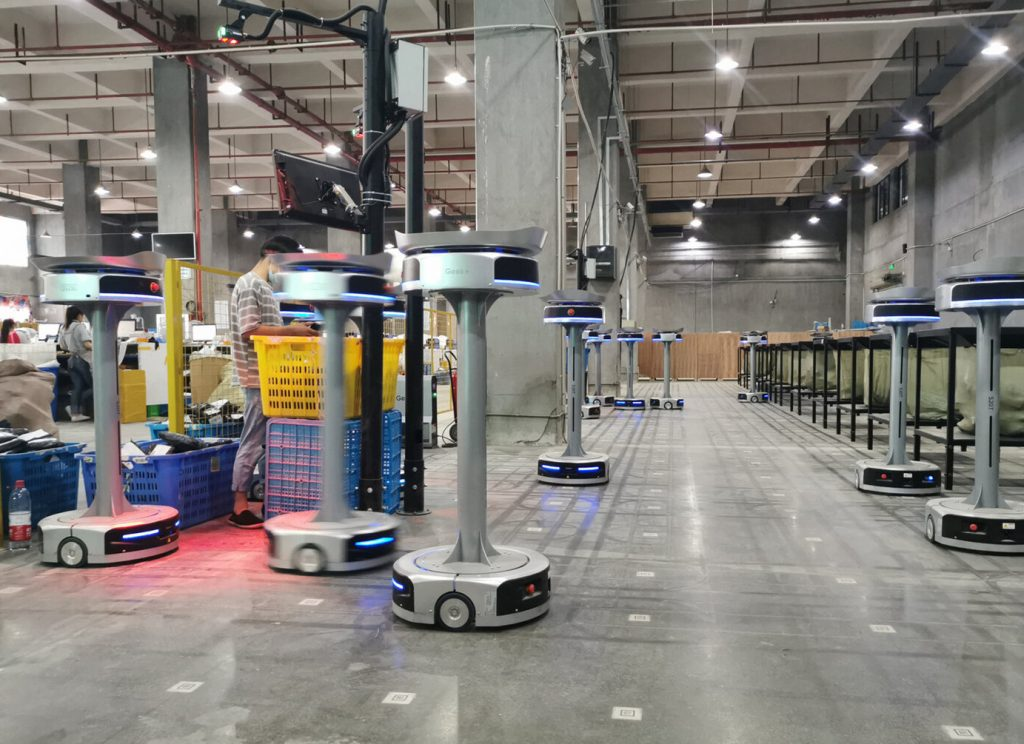
\includegraphics[width=14cm]{assets/amr_sort.jpg}
    \caption{Exemple d'un robot autonome pour le tri des stocks \cite{LargescaleAMRSorting2020}}
    \label{amr_sort}
    \end{figure}




Leur flexibilité leur permet également d’intervenir dans une multitude d’autres domaines, comme le transport, les services et les établissements de santé.


\section{Caracteristiques des robot mobile}
Les robots Meanwhile sont dotés de l’intelligence artificielle spécialisée dans la navigation en intérieur (SLAM). Le SLAM, Simultaneous Localisation And Mapping, permet au robot de construire son environnement et de modifier son comportement en fonction des obstacles non cartographiés tout en se localisant en temps réel. Afin de se déplacer en toute autonomie et sans trajectoire prédéfinie, le robot va combiner les informations qui lui sont propre avec les informations de son environnement (renvoyées par ses lasers et capteurs .)

 Pour être considéré comme tel, un AMR doit répondre aux caractéristiques suivantes :

Planification de mouvement
Pour réaliser sa mission, l’AMR a la capacité d’optimiser son trajet. Sa configuration de départ va définir sa trajectoire globale et va évoluer en fonction des données récupérées en temps réel ce qui va altérer sa trajectoire locale. L’AMR va ainsi calculer, en permanence, son chemin sans collision. En d’autres termes, pour réaliser sa mission, le robot Meanwhile optimise son trajet, qu’il a lui-même défini au départ (trajectoire globale), tout en évitant les obstacles qui se présentent éventuellement à lui (trajectoire locale).

Localisation
Pour pouvoir planifier son trajet en toute autonomie, les robots mobiles Meanwhile sont en mesure de se localiser dans leur environnement. Ils utilisent un certain nombre de capteurs embarqués, tel que des scrutateurs lasers, lasers verticaux etc. Pour être en permanence localisés, les robots Meanwhile vont, en temps réel, comparer leur cartographie à l’environnement modélisé par leurs capteurs. Ainsi, tout défaut de positionnement intrinsèque est instantanément corrigé et le robot est en permanence localisé.Par ailleurs, lorsque les environnements de travail sont très dynamiques, il est possible d’améliorer la localisation du robot par un système de triangulation lumineuse, appelé Acuity.

Navigation naturelle 
Les robots mobiles sont en mesure de calculer les commandes des actionneurs du système permettant de réaliser le mouvement planifié. Le robot planifie sa propre trajectoire. Il suit le chemin prévu (trajectoire globale) tout en évitant les obstacles non cartographiés sur le chemin. Si le robot rencontre des obstacles, il modifie sa trajectoire « locale » pour les éviter mais si ce dernier ne peut pas continuer (par exemple, une porte est fermée), il replanifie globalement son trajet (par exemple, trouver une porte différente.)

Évitement réactif d’obstacles 
En complément du scrutateur laser principal de sécurité, situé à 200mm du sol, les cobots mobiles Meanwhile sont équipés de différents capteurs leurs permettant de contourner et d’éviter les obstacles :

Un scrutateur laser de « détection de pieds » situé à 60mm du sol. Ce capteur permet au Cobot Mobile de détecter et de contourner tout obstacle situé au niveau du sol.

Une rangée de sonars situés à l’arrière du Cobot Mobile. Ces capteurs permettent un mouvement de recul sécuritaire du Cobot Mobile. A noter que le Cobot Mobile ne recule que dans des zones identifiables et jamais de sa propre initiative (appel d’une fonction au cours d’une séquence) (accostage de la station de charge par exemple).

Les scrutateurs lasers verticaux, permettant de créer deux plans de part et d’autre du Cobot Mobile. Il peut alors détecter de manière fiable tout objet surplombant situé dans un plan différent des scrutateurs horizontaux (fourches de chariots élévateurs, tablettes opérateur, etc…) ainsi que toute déclivité dans le sol. Ces données sont utilisées lors de la navigation et permettent au Cobot Mobile de se mouvoir de façon optimale entre les obstacles dans des environnements complexes.

Déploiement rapide 
L’installation des robots mobiles autonomes Meanwhile est réalisée dans des délais extrêmement courts car il n’est pas nécessaire de modifier l’infrastructure existante. De même que les robots peuvent être reprogrammés facilement, si l’infrastructure et le besoin évoluent. (Nos clients sont en mesure de modifier eux-mêmes les points de livraisons.)

\section{Structure de la commande d’un robot mobile}
%https://www.ummto.dz/dspace/bitstream/handle/ummto/7624/LamaraNabil.pdf?sequence=1&isAllowed=y
L'objectif de la robotique est d'atteindre un objectif dans son environnement en évitant les obstacles. Le problème que l'on doit résoudre est de déterminer les commandes appropriées en fonction des données capteurs qu'elles commandent doivent être envoyées à chaque instant au robot pour atteindre cet objectif. Donc l'idée est de permettre au robot d'évoluer dans un monde prévue à l'origine pour l'homme. 


\subsection{Perception et modélisation de l'environnement}

Le robot doit être muni d’un système de perception capable de fournir des informations précises sur l'état de l’environnement qui l’entoure, afin de pouvoir identifier et regrouper des éléments utiles pour une représentation fiable et consistante de cet environnement.
\begin{figure}[h]
    \centering
    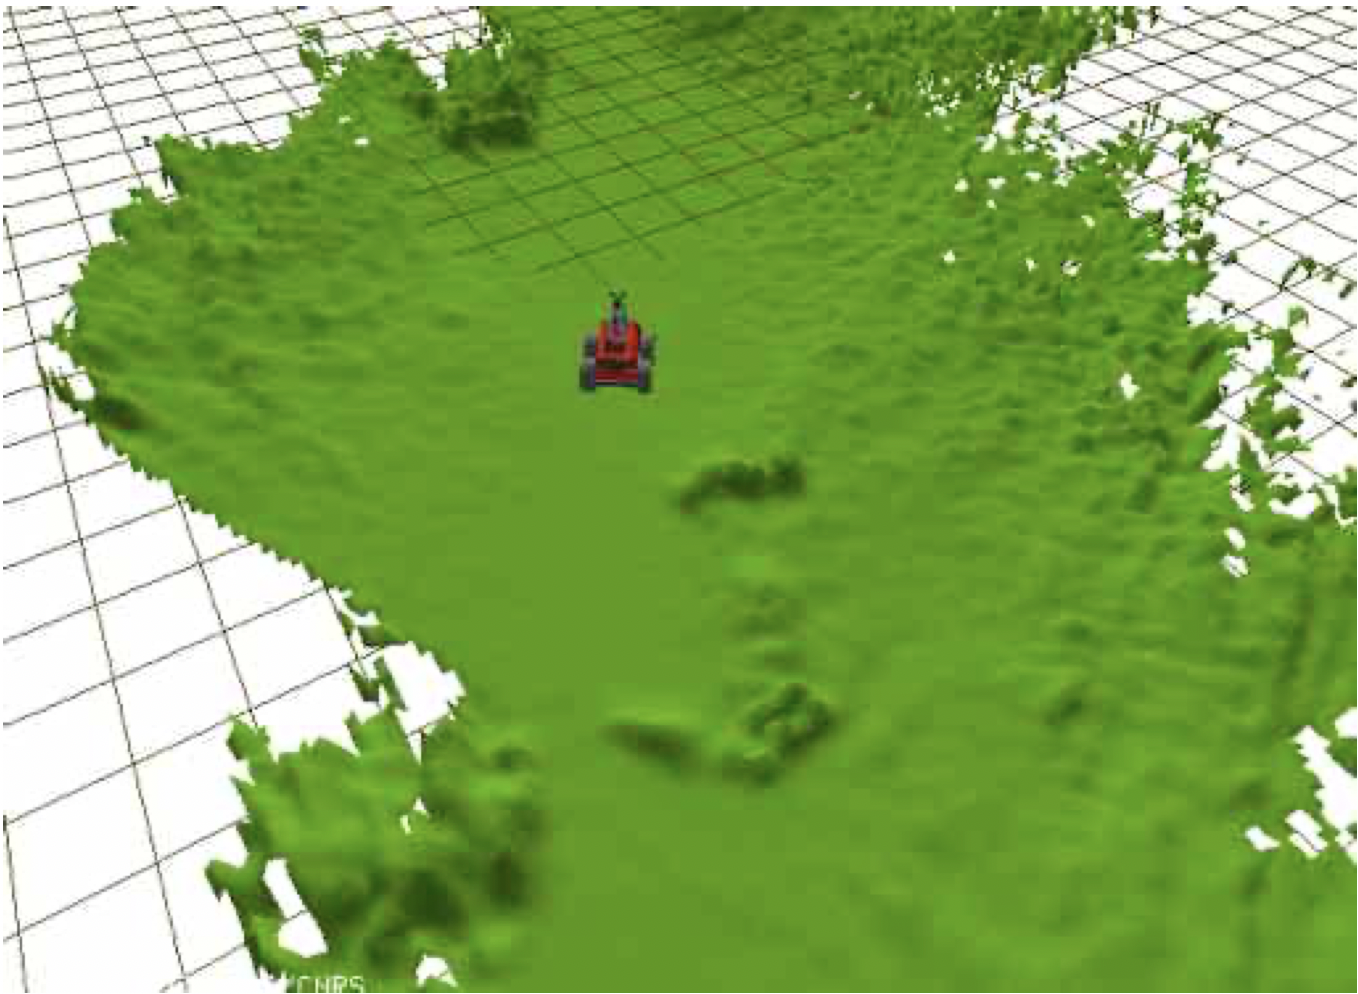
\includegraphics[width=14cm]{assets/perception.png}
    \caption{Exemple de la perception d'un robot mobile }
    \label{perception}
    \end{figure}

\subsection{Communication homme machine}

La communication machine est très essentielle pour cela des interfaces de plus en plus conviviale sont développés.
La communication est réalisée à l’aide de multiples supports : écrit, visuel, ou encor sonore. Le module de communication semble prendre de plus en plus d’importance à l’heure actuelle.
\subsection{Commande}

Architecture traditionnelle de décomposition du programme de contrôle du robot en différents modules de fonctionnement est donnée comme suit :
caoture decean 

Du monde abstrait au monde concret, la planification des actions et le contrôle des déplacements se situent dans le monde idéal, monde perçu et le monde réel cette décomposition est classique pour les systèmes automatiques de commande.
\section{Navigation autonome d’un robot mobile
}
Généralement, la navigation d’un robot mobile est une tâche qui consiste à trouver un mouvement libre dans l’espace de configuration sans collision avec les obstacles proche du robot. Ce mouvement amène le robot d’une configuration initiale, vers une position finale désirée.
Le robot mobile doit mettre en œuvre certains nombres de fonctionnalités pour exécuter une tâche de navigation autonome :
\subsection{Localisation}

Le succès dans l’exécution d’une tâche associée à un déplacement est directement lié à la capacité des robots de se positionner par rapport à son environnement. Cette localisation doit être la plus précise possible, et dépend de la fiabilité, de la représentation de l’environnement construite par le système et de la perception du robot.
\subsection{Planification et exécution de mouvements}

Le robot doit être capable de se déplacer de façon sûre à travers l’espace libre de l’environnement, tenant compte de la présence d’éventuels obstacles statiques et dynamiques. Le problème de déplacement du robot dans l’environnement rencontre les mêmes difficultés que la localisation et la modélisation liées à la présence d’incertitudes qui font que le déplacement commandé ne sera pas de manière générale exécuté parfaitement.
Ces fonctions ne sont pas indépendantes. On note, bien évidemment, que la perception de l’environnement intervient dans toutes. La planification de mouvement s’intéresse au calcul automatique de chemins sans collision pour un robot quelconque (robot mobile, bras manipulateur, etc.) évoluant dans un environnement encombrés d’obstacles.Historiquement les premières études ont été basées sur le cycle classique en intelligence artificielle : perçoit, pense, agit.
La décomposition du problème a été à l’origine de nombreux travaux. La présence de multiples modules attachés chacun à la résolution d’un sous problème nécessite la mise en place d’une organisation permettant la construction d’un système complexe à partir ces briques élémentaires. Cette organisation est appelée architecture de contrôle.
\subsection{Suivi de trajectoire
}
Cette étape consiste à calculer les commandes des actionneurs du système permettant de réaliser le mouvement planifié. Un robot étant considéré comme un système dynamique. [On utilise des méthodes de commande à retour d’état pour l’asservissement de système sur une trajectoire de référence].
\subsection{Evitement d’obstacles et parking
}

L’évitement des obstacles est un comportement de base présent quasiment dans tous les mouvements des robots mobiles. Cependant pour des anomalies comme une localisation imparfaite, le suivi de la trajectoire planifiée ne garantie pas l’absence de collision avec les objets statique ou dynamique existant.
L’étape finale de la navigation autonome s’appelle Parking, elle nécessite une forte précision pour l’atteinte du bute finale.






\chapter{Systéme de vision et calibrage de cameras}

\chapter{Résultats et simulation}


%\chapter{Conclusion génerale}

\newpage
\input{Parts/conclusion.tex}
\bibliography{bib.bib}
\bibliographystyle{plain}
\input{Parts/resume.tex}
\printglossaries
\end{document}